\documentclass[12pt,letterpaper]{article}

% -------------------- Paquetes --------------------
\usepackage[utf8]{inputenc}
\usepackage[T1]{fontenc}
\usepackage[spanish]{babel}
\usepackage{geometry}
\geometry{margin=2.5cm}
\usepackage{setspace}
\onehalfspacing
\usepackage{graphicx}
\usepackage{float}
\usepackage{caption}
\usepackage{subcaption}
\usepackage{siunitx}
\sisetup{detect-all, round-mode=places, round-precision=3}
\usepackage{hyperref}
\usepackage{xcolor}
\usepackage{fancyhdr}
\usepackage{tikz}
\usepackage{eso-pic}
\usepackage{booktabs}
\usepackage{tabularx}
\usepackage{array}
\usepackage{amsmath}
\usepackage{amssymb}
\usepackage{listings}

\hypersetup{colorlinks=true, linkcolor=blue, urlcolor=blue}

% -------------------- Listings (VHDL) --------------------
\lstdefinelanguage{VHDL}{
  morekeywords=[1]{library,use,all,entity,is,port,in,out,end,architecture,of,begin,process,signal,if,then,elsif,rising_edge,else,when,others,generic,map,case,variable,for,loop,nor,xor,and,or,not,downto,to,wait,constant,type,array},
  morekeywords=[2]{std_logic,std_logic_vector,signed,unsigned,integer,std_logic_1164,numeric_std,time},
  sensitive=true,
  morecomment=[l]{--},
  morestring=[b]"
}
\lstset{
  language=VHDL,
  basicstyle=\ttfamily\small,
  frame=single,
  numbers=left,
  numberstyle=\tiny,
  breaklines=true,
  tabsize=2,
  captionpos=b
}

% -------------------- Encabezado / Pie --------------------
\pagestyle{fancy}
\fancyhf{}
\lhead{\textbf{P26-LIS2022-1}}
\rhead{\textbf{Práctica 3:} Memorias ROM y RAM}
\renewcommand{\headrulewidth}{0.4pt}

\fancyfoot[C]{\small
\begin{tabular}{c}
186028; \href{mailto:robbie.curiosodr@udlap.mx}{robbie.curiosodr@udlap.mx}
\end{tabular}
}
\fancyfoot[R]{\small \thepage}

% -------------------- Marca de agua UDLAP --------------------
\AddToShipoutPictureBG{%
  \begin{tikzpicture}[remember picture,overlay]
    \node[opacity=0.08, rotate=12, anchor=south east] at ([xshift=1.8cm,yshift=-1.6cm]current page.south east)
    {
\includegraphics[width=0.75\paperwidth]{udlap_logo.png}};
  \end{tikzpicture}
}

\setlength{\parskip}{6pt}
\setlength{\parindent}{0pt}

\newcolumntype{L}[1]{>{\raggedright\arraybackslash}p{#1}}
\newcolumntype{C}[1]{>{\centering\arraybackslash}p{#1}}

\graphicspath{{../imagenes/}}

\begin{document}

% ========================= PORTADA =========================
\begin{titlepage}
\thispagestyle{empty}
\begin{center}
\vspace*{0.8cm}

{\Large \textsc{Universidad de las Américas Puebla}}\par
{\small Departamento de Computación, Electrónica y Mecatrónica}\par

\vspace{1.2cm}

{\Huge \textbf{Reporte de práctica}}\par
\vspace{0.15cm}
{\Large \textbf{Práctica 3: Memorias ROM y RAM para la Tarjeta PYNQ Z1}}\par

\vspace{1.0cm}

\begin{minipage}{0.92\textwidth}
\rule{\textwidth}{0.8pt}\par
\vspace{0.35cm}

\begin{tabular}{@{}L{0.30\textwidth}L{0.62\textwidth}@{}}
\textbf{Materia} & P26-LIS2022-1\\
& Arquitecturas Computacionales\\
\textbf{Profesor} & Dr. Omar Guillén Fernández\\
\textbf{Sección} & 2\\
\textbf{Periodo} & Primavera 2026\\
\end{tabular}

\vspace{0.35cm}
\rule{\textwidth}{0.8pt}
\end{minipage}

\vfill

\begin{minipage}{0.92\textwidth}
\textbf{Integrante}\par
\vspace{0.25cm}
Robbie Nicolás Curioso de Salazar \hfill 186028 \hfill \href{mailto:robbie.curiosodr@udlap.mx}{robbie.curiosodr@udlap.mx}\par
\end{minipage}

\vspace{0.6cm}

\end{center}
\end{titlepage}

% ========================= CONTENIDO =========================
\section{Introducción}
Las memorias son uno de los bloques esenciales de cualquier sistema digital: almacenan tanto las instrucciones que ejecuta un procesador como los datos que éste procesa. En esta práctica se diseñaron e implementaron, en VHDL, dos tipos de memorias síncronas pensadas para sintetizarse sobre la tarjeta PYNQ~Z1, que está basada en el SoC Zynq~7000 (FPGA + procesador ARM): una memoria ROM con datos de cumpleaños, y una memoria RAM para almacenar fechas de nacimiento.

Adicionalmente, se planteó el uso de memorias ROM como almacén de programas escritos en lenguaje ensamblador RISC-V, como continuación de la Tarea~3. Para ello se discuten tres pequeños programas: el cálculo de $(a+b)\cdot c$, el factorial de cinco y la detección de paridad de un entero, junto con su codificación binaria en RV32I que se grabaría en cada ROM.

La verificación funcional se realizó mediante simulación en \textit{Active-HDL} con un banco de pruebas que ejercita la lectura de la ROM de cumpleaños y la escritura/lectura de la RAM de fechas.

\section{Objetivos}
\begin{itemize}
  \item Implementar en VHDL una memoria ROM síncrona inicializada con datos en código, configurable mediante \textit{generics} de ancho de dirección y ancho de dato.
  \item Implementar una memoria RAM síncrona de un puerto, con escritura controlada por \texttt{we} y lectura registrada.
  \item Cargar la ROM con cumpleaños de compañeros del curso en formato BCD (DDMM) y la RAM con fechas de nacimiento de 32 bits en formato DDMMYYYY.
  \item Discutir el uso de memorias ROM como almacén de programas RV32I, presentando el ensamblador y la codificación hexadecimal de los tres programas planteados en la Tarea~3.
  \item Validar el comportamiento síncrono de ambas memorias mediante simulación en Active-HDL y diagramas de tiempo.
\end{itemize}

\section{Materiales y herramientas}
\begin{itemize}
  \item \textbf{Software:} Active-HDL Student Edition para compilación y simulación funcional.
  \item \textbf{Lenguaje:} VHDL, con uso de las bibliotecas \texttt{ieee.std\_logic\_1164} y \texttt{ieee.numeric\_std}.
  \item \textbf{Tecnología objetivo:} Zynq~7000 sobre tarjeta PYNQ~Z1 (referencia para discutir la inferencia de bloques BRAM).
  \item \textbf{Documentación:} guía oficial de la práctica, documentos UG585 y UG953 de Xilinx, y la especificación RV32I de RISC-V para la sección de Tarea~3.
\end{itemize}

\section{Marco teórico}

\subsection{Memoria ROM}
Una ROM (\textit{Read-Only Memory}) es una memoria de solo lectura cuyo contenido queda fijado en el momento del diseño. En VHDL se modela como un arreglo constante indexado por una dirección. Para que el sintetizador la reconozca como memoria distribuida o como bloque BRAM dentro de la FPGA, la lectura se realiza dentro de un proceso síncrono al reloj, lo cual introduce un retardo de un ciclo entre la presentación de la dirección y la aparición del dato en la salida.

\subsection{Memoria RAM de un puerto}
Una RAM síncrona de un puerto admite escritura y lectura sobre la misma dirección, sincronizadas con el flanco de subida del reloj. Cuando la señal de habilitación \texttt{we} se encuentra en alto, el dato presentado en \texttt{data\_in} se almacena en la posición indicada; en cualquier otro caso, la salida \texttt{data\_out} entrega el dato de la dirección registrada en el ciclo anterior. Esta convención es la que recomienda Xilinx para inferir BRAMs en la familia 7~Series.

\subsection{Bloques BRAM en el Zynq 7000}
El Zynq~7000 que monta la PYNQ~Z1 cuenta con bloques de memoria dedicados (BRAM) de 36~Kb cada uno, distribuidos en columnas dentro del tejido de la FPGA. Cuando un diseño VHDL describe una memoria síncrona con un patrón estándar de lectura/escritura, el sintetizador (Vivado) infiere automáticamente uno o varios BRAMs para implementarla. Para profundidades pequeñas (decenas de palabras), el sintetizador puede optar por lógica distribuida (LUTs configurados como pequeñas memorias) en lugar de un BRAM completo.

\subsection{Codificación de instrucciones RV32I}
Cada instrucción RISC-V de 32 bits se compone de campos fijos. Las instrucciones de tipo I, como \texttt{ADDI} o \texttt{ANDI}, tienen el formato \mbox{\texttt{imm[11:0] | rs1 | funct3 | rd | opcode}}. Las instrucciones de tipo R, como \texttt{ADD}, agregan los campos \texttt{funct7} y \texttt{rs2}. Para los corrimientos con inmediato (\texttt{SLLI}), el campo inmediato se interpreta como una cantidad de cinco bits ubicada en \texttt{imm[4:0]}, junto con \texttt{funct7=0000000}.

\section{Diseño y procedimiento}

\subsection{Memoria ROM de cumpleaños}
Se describió la entidad \texttt{rom\_cumpleanos} con dos genéricos: \texttt{addr\_width} y \texttt{data\_width}. Para la práctica se fijó \texttt{addr\_width=4} (16 posiciones) y \texttt{data\_width=16} (suficientes para empacar día y mes en BCD). El contenido de la memoria se declara como una constante de tipo arreglo, donde cada entrada lleva el formato \texttt{0xDDMM}, por ejemplo \texttt{0x1505} representa el 15 de mayo. La lectura se hace dentro de un proceso síncrono al reloj que copia el dato direccionado a una señal interna, la cual luego se propaga a la salida \texttt{data\_out}.

\subsection{Memoria RAM de fechas de nacimiento}
La entidad \texttt{ram\_fechas} sigue una estructura similar pero con \texttt{data\_width=32} para almacenar fechas en formato \texttt{0xDDMMYYYY}. La memoria se modela con una señal interna inicializada a cero (lo cual permite verificar su estado inicial en simulación). Dentro del proceso síncrono se evalúa la señal \texttt{we}: si está en alto, se escribe el dato de entrada en la posición indicada; en cualquier caso, la dirección se registra en una señal auxiliar \texttt{read\_addr}, y la salida combinacional \texttt{data\_out} se obtiene leyendo la posición indicada por \texttt{read\_addr}. Este patrón es estándar para inferir BRAMs y produce un retardo de un ciclo en la lectura.

\subsection{Banco de pruebas}
El testbench \texttt{tb\_memorias} instancia tanto la ROM de cumpleaños como la RAM de fechas, genera un reloj con período de \SI{10}{\nano\second} y aplica los siguientes estímulos:

\begin{enumerate}
  \item Recorrido completo de la ROM, leyendo las direcciones $0$ a $15$ con un ciclo por dirección.
  \item Cinco escrituras en la RAM con \texttt{we=1}: la fecha \texttt{0x15052003} en la posición 0, \texttt{0x22082002} en 1, \texttt{0x07122003} en 5, \texttt{0x14112002} en 10 y \texttt{0x30012004} en 15.
  \item Recorrido completo de la RAM con \texttt{we=0}, leyendo las posiciones $0$ a $15$ para verificar tanto las direcciones escritas como las que permanecen en cero.
\end{enumerate}

\subsection{Flujo en Active-HDL}
Para cada simulación se siguió el procedimiento habitual:
\begin{enumerate}
  \item Crear el espacio de trabajo y agregar los archivos \texttt{rom\_cumpleanos.vhd}, \texttt{ram\_fechas.vhd} y \texttt{tb\_memorias.vhd}.
  \item Compilar primero las dos memorias y, finalmente, el banco de pruebas.
  \item Inicializar la simulación con \texttt{tb\_memorias} como nivel superior.
  \item Agregar al \textit{waveform} las ocho señales de interés (\texttt{clk}, \texttt{cump\_addr}, \texttt{cump\_data\_out}, \texttt{ram\_we}, \texttt{ram\_addr}, \texttt{ram\_data\_in}, \texttt{ram\_data\_out}) y configurar el formato hexadecimal para las señales de datos y binario para las direcciones.
  \item Ejecutar \textit{Run For} con duración de \SI{400}{\nano\second}.
\end{enumerate}

\section{Resultados y discusión}

La Figura \ref{fig:general} muestra la simulación completa, donde se aprecian las dos fases: la primera mitad corresponde al recorrido de la ROM de cumpleaños y la segunda mitad al ciclo de escritura y lectura de la RAM de fechas. En las subsecciones siguientes se analiza cada bloque por separado.

\begin{figure}[H]
\centering

\includegraphics[width=\textwidth]{sim_general.png}
\caption{Vista panorámica de la simulación: lectura de la ROM seguida de escritura y lectura de la RAM.}
\label{fig:general}
\end{figure}

\subsection{ROM de cumpleaños}
La Figura \ref{fig:rom_cump} muestra la lectura secuencial de las dieciséis direcciones de la ROM. Conforme la dirección \texttt{cump\_addr} avanza de \texttt{0000} hasta \texttt{1111}, la salida \texttt{cump\_data\_out} entrega el cumpleaños correspondiente con un ciclo de retraso, lo cual confirma que la ROM funciona como memoria síncrona.

\begin{table}[H]
\centering
\caption{Contenido de la ROM de cumpleaños (formato BCD: \texttt{0xDDMM}).}
\label{tab:cumpleanos}
\begin{tabular}{C{1.2cm}C{2cm}C{3cm}}
\toprule
Dirección & Valor (hex) & Fecha (DD/MM)\\
\midrule
0  & \texttt{1505} & 15/05\\
1  & \texttt{2208} & 22/08\\
2  & \texttt{0712} & 07/12\\
3  & \texttt{3001} & 30/01\\
4  & \texttt{1411} & 14/11\\
5  & \texttt{0904} & 09/04\\
6  & \texttt{1806} & 18/06\\
7  & \texttt{0211} & 02/11\\
8  & \texttt{2503} & 25/03\\
9  & \texttt{1207} & 12/07\\
10 & \texttt{0509} & 05/09\\
11 & \texttt{2802} & 28/02\\
12--15 & \texttt{0000} & --\\
\bottomrule
\end{tabular}
\end{table}

Las posiciones \texttt{12} a \texttt{15} se dejaron en cero para reflejar el comportamiento de una ROM con menos entradas que su capacidad nominal: las direcciones no inicializadas explícitamente devuelven el valor por defecto. Esto es consistente con la práctica común de declarar una ROM más grande que el contenido para dejar espacio a futuras adiciones.

\begin{figure}[H]
\centering
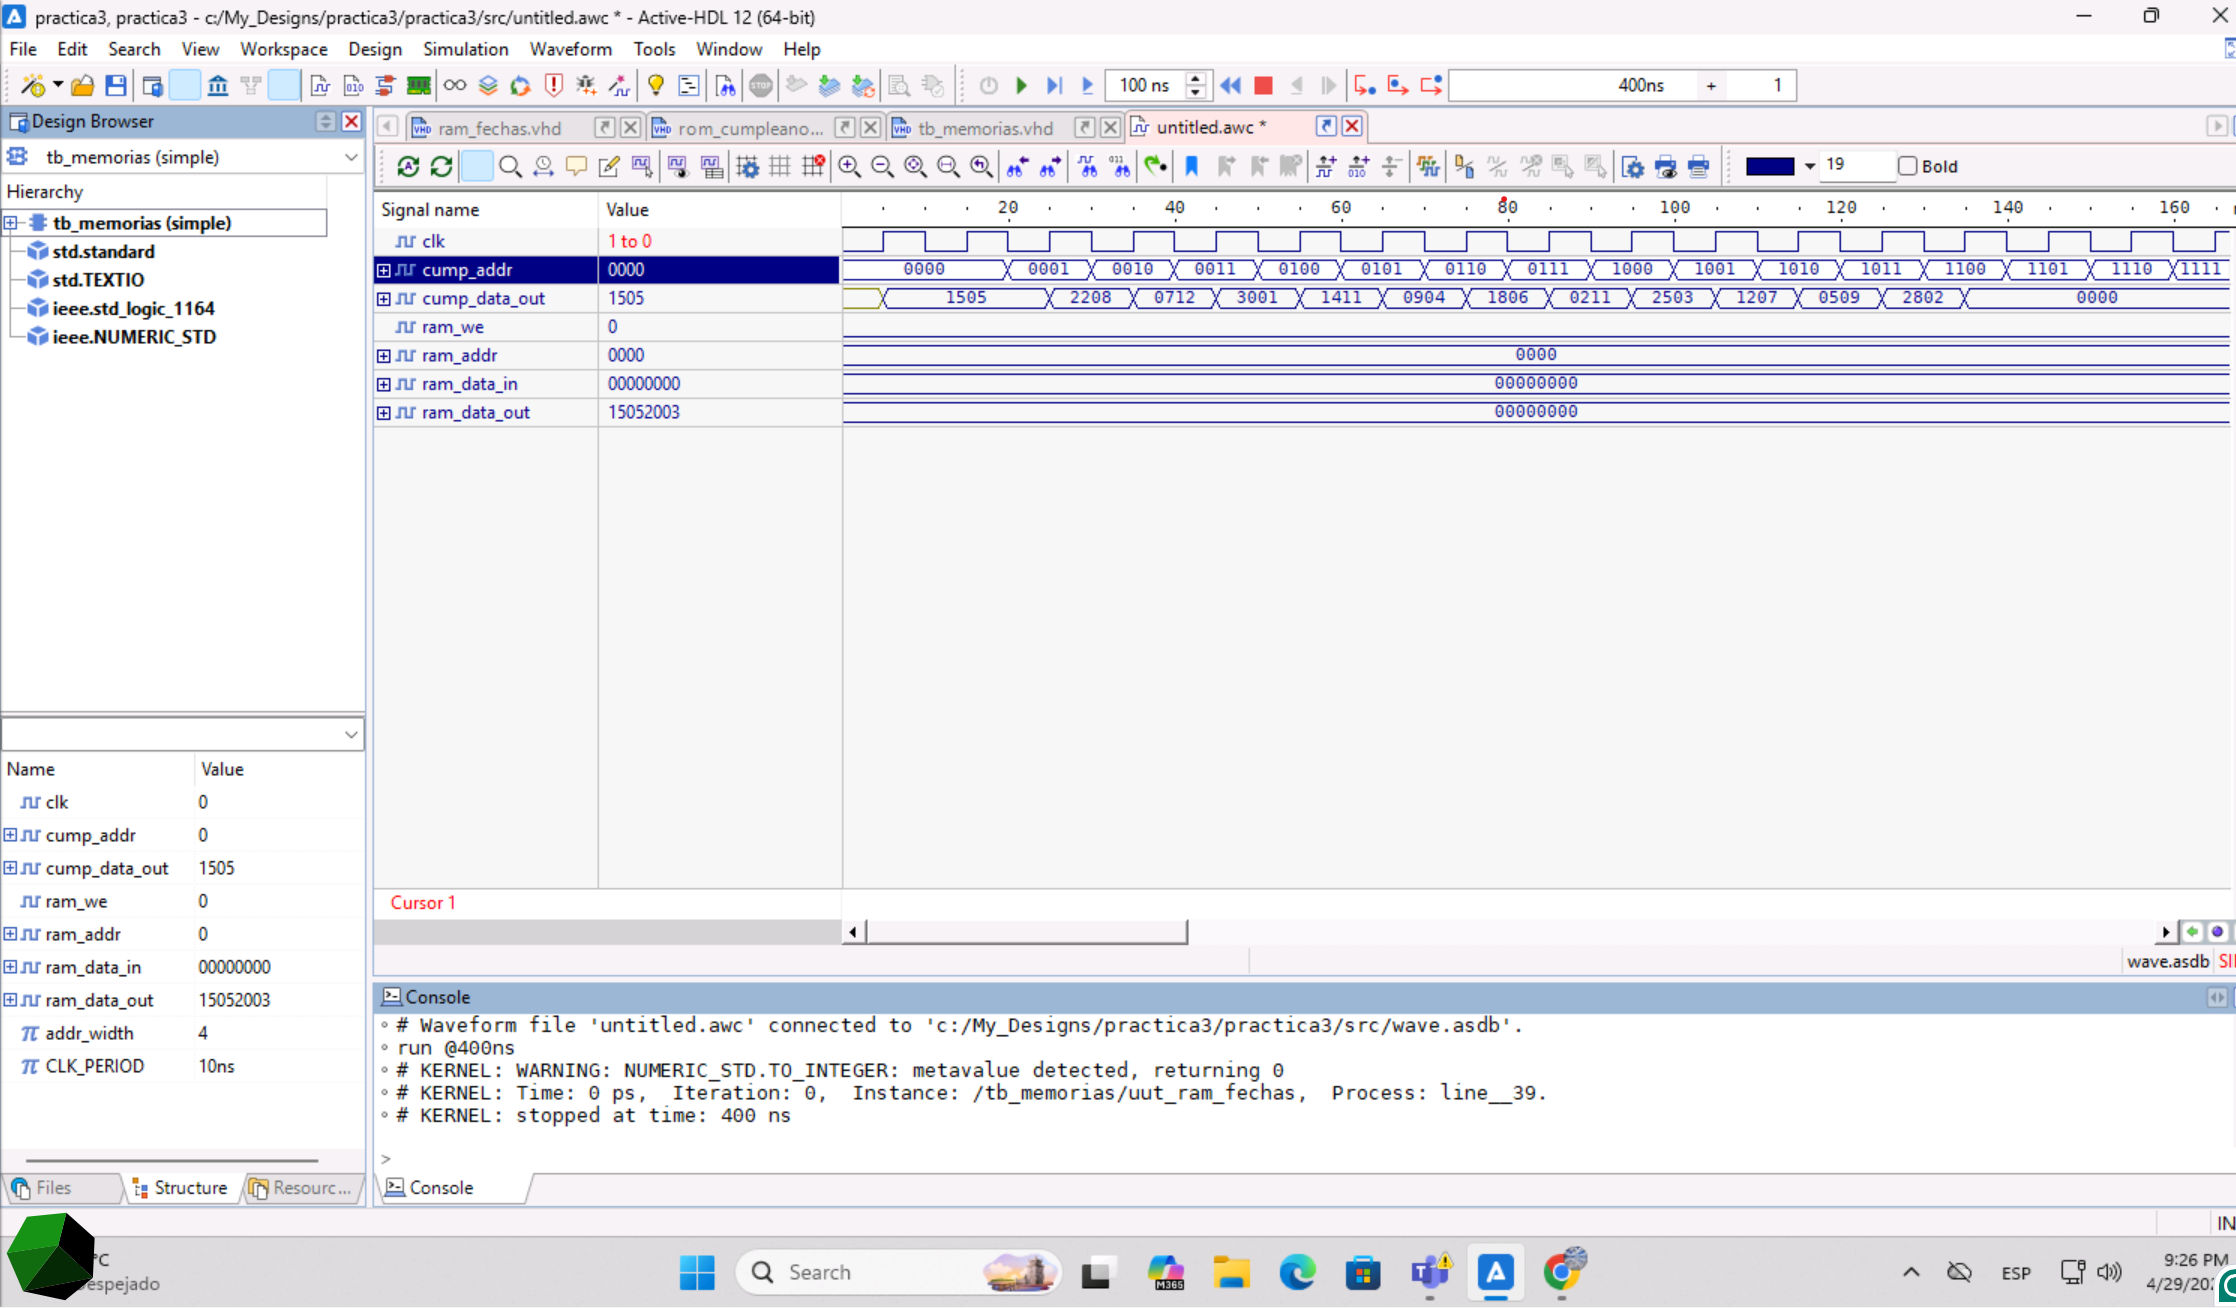
\includegraphics[width=\textwidth]{sim_cumpleanos.png}
\caption{Lectura de las dieciséis direcciones de la ROM de cumpleaños.}
\label{fig:rom_cump}
\end{figure}

\subsection{RAM de fechas de nacimiento}
La Figura \ref{fig:ram} concentra las dos fases de la RAM. Durante la primera región la señal \texttt{ram\_we} permanece en alto y se aplican cinco vectores de entrada: \texttt{0x15052003}, \texttt{0x22082002}, \texttt{0x07122003}, \texttt{0x14112002} y \texttt{0x30012004}, dirigidos a las posiciones 0, 1, 5, 10 y 15 respectivamente. En la segunda región \texttt{ram\_we} baja a cero y la dirección recorre las dieciséis posiciones; la salida \texttt{ram\_data\_out} entrega los valores escritos en las cinco direcciones modificadas y devuelve cero en las demás, confirmando tanto la inicialización a cero como la persistencia de los datos almacenados.

\begin{figure}[H]
\centering
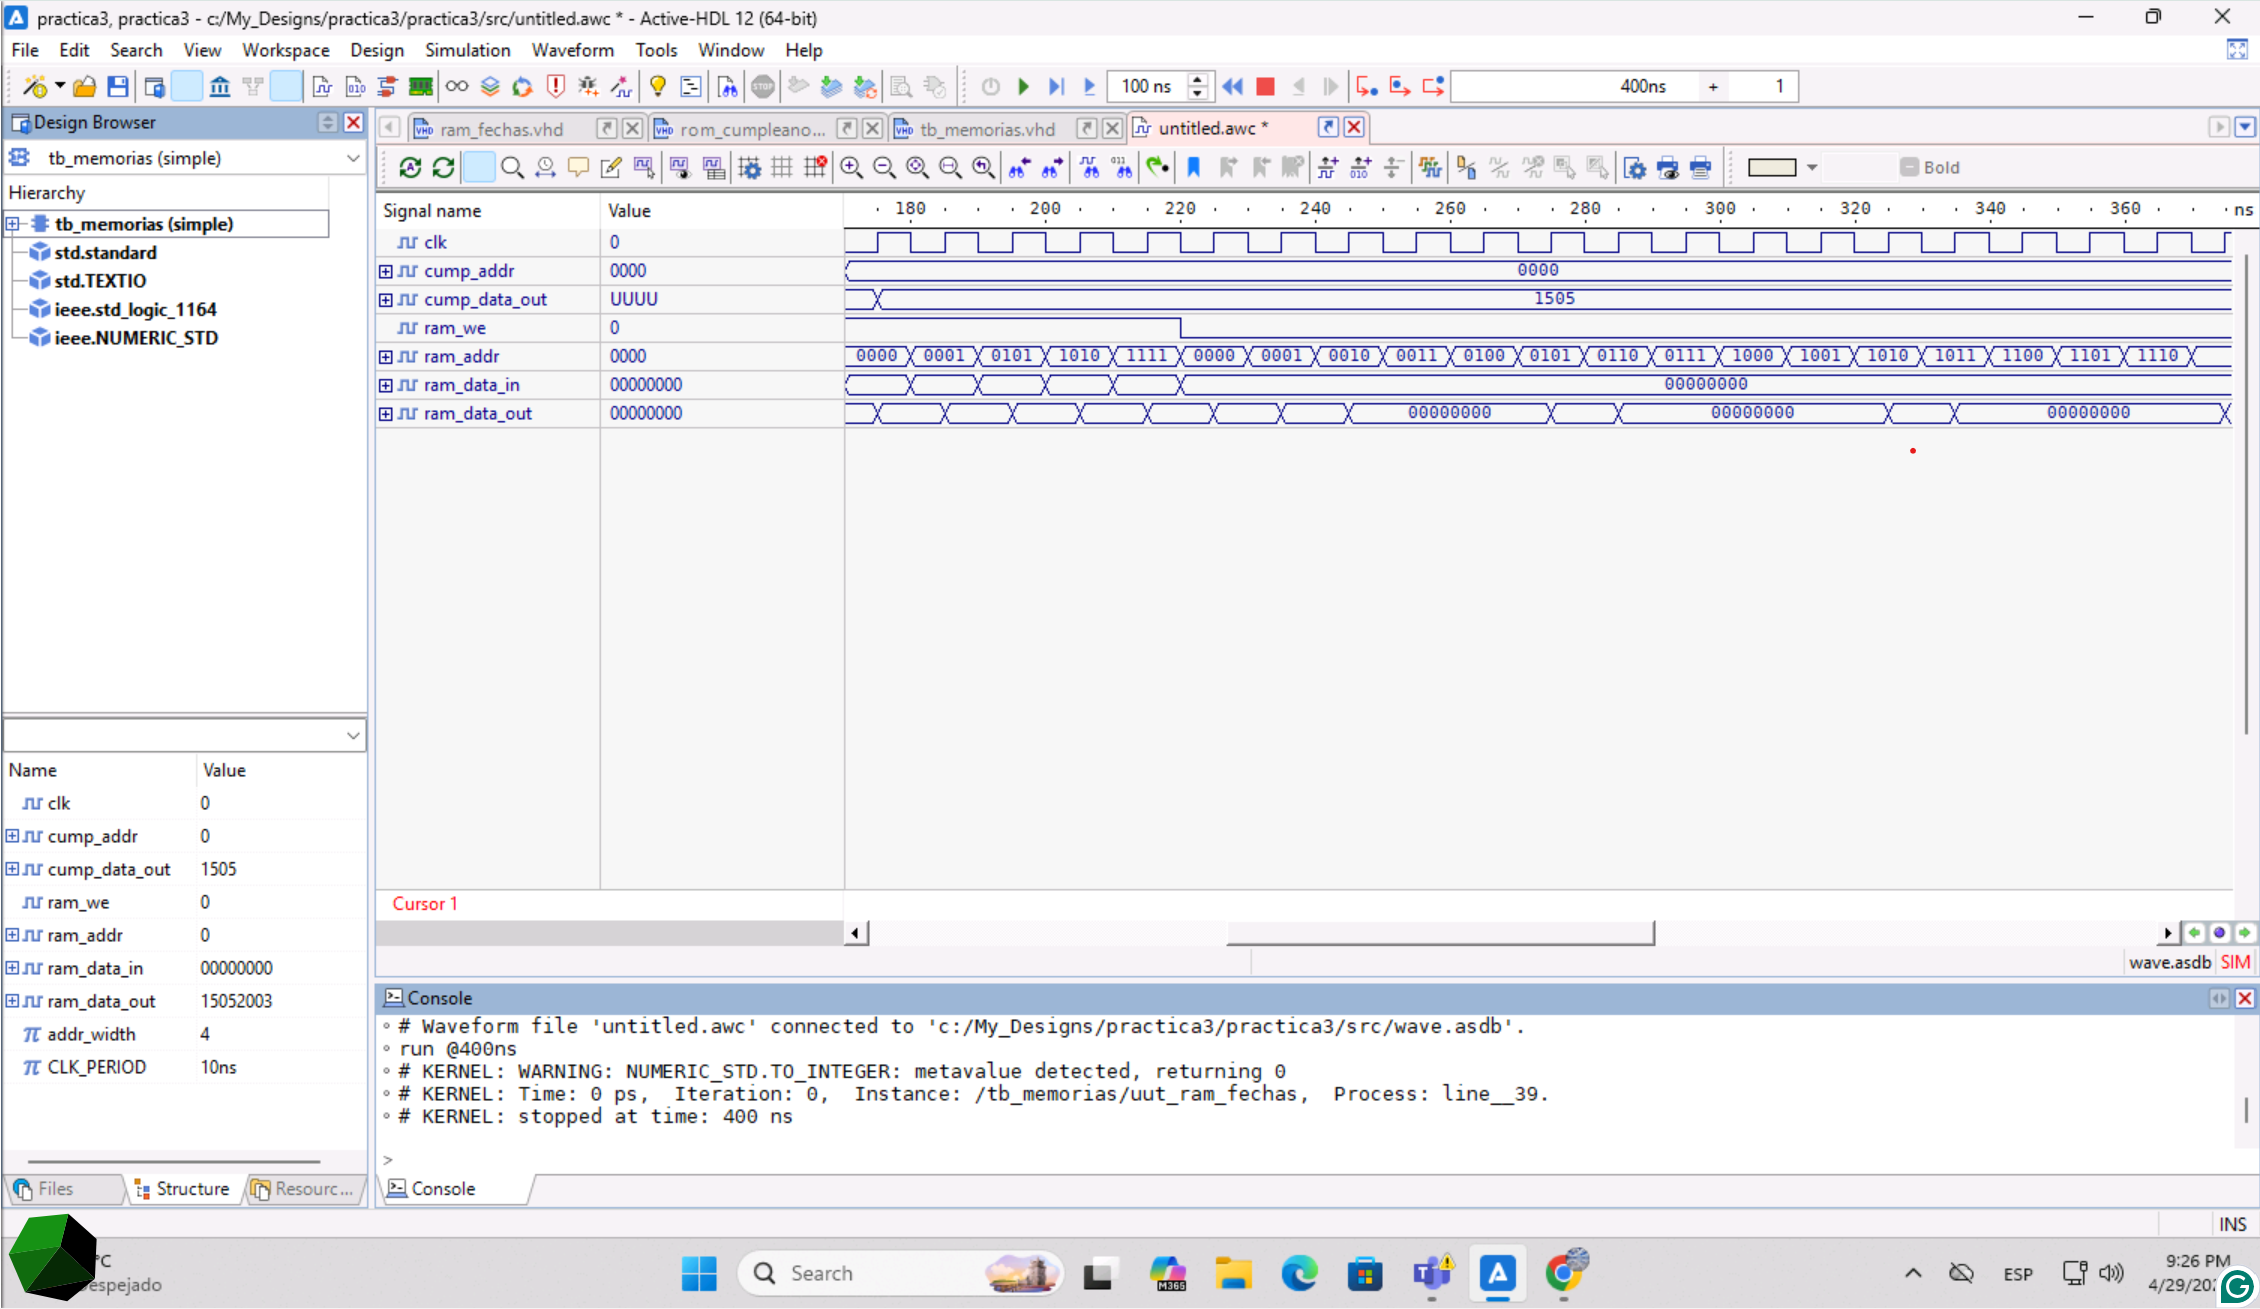
\includegraphics[width=\textwidth]{sim_ram.png}
\caption{Operación de la RAM de fechas: ciclo de escritura seguido de lectura completa.}
\label{fig:ram}
\end{figure}

Es importante notar el retardo de un ciclo entre la presentación de una dirección y la aparición del dato en la salida. Este retardo es propio de la arquitectura síncrona y proviene del registro intermedio (\texttt{read\_addr}) que se utiliza para que el sintetizador infiera correctamente un BRAM. En un sistema completo, este retardo debe tenerse en cuenta al conectar la RAM a una unidad de control: la señal de validez del dato leído está disponible un ciclo después de la dirección.

\subsection{ROMs de la Tarea 3}
Adicionalmente al uso de la ROM como almacén de datos, se planteó como ejercicio cargar tres pequeños programas escritos en RV32I dentro de memorias ROM independientes. Estas ROMs no se simulan en este banco de pruebas, pero se documenta su contenido para complementar la discusión.

\subsubsection{ROM de \texorpdfstring{$(a+b)\cdot c$}{(a+b)*c}}
El programa calcula $(5+5)\cdot 4 = 40$ usando un corrimiento a la izquierda en lugar de una multiplicación, ya que el conjunto base RV32I no incluye \texttt{MUL}. La secuencia de cinco instrucciones se muestra en la Tabla \ref{tab:abc}.

\begin{table}[H]
\centering
\caption{Programa RV32I para $(a+b)\cdot c$ con $a=5$, $b=5$, $c=4$.}
\label{tab:abc}
\begin{tabular}{C{1.2cm}C{4cm}C{3cm}C{4.5cm}}
\toprule
Dirección & Ensamblador & Hex & Significado\\
\midrule
0 & \texttt{addi x1, x0, 5}  & \texttt{0x00500093} & $x_1 \leftarrow 5$\\
1 & \texttt{addi x2, x0, 5}  & \texttt{0x00500113} & $x_2 \leftarrow 5$\\
2 & \texttt{addi x3, x0, 4}  & \texttt{0x00400193} & $x_3 \leftarrow 4$\\
3 & \texttt{add  x4, x1, x2} & \texttt{0x00208233} & $x_4 \leftarrow x_1+x_2 = 10$\\
4 & \texttt{slli x5, x4, 2}  & \texttt{0x00221293} & $x_5 \leftarrow x_4\ll 2 = 40$\\
\bottomrule
\end{tabular}
\end{table}

El resultado final, $x_5 = 40$, queda almacenado en el registro \texttt{x5}. El uso del corrimiento a la izquierda por dos posiciones equivale a multiplicar por $4$, lo cual aprovecha el hecho de que $c$ es una potencia de $2$.

\subsubsection{ROM del factorial de cinco}
El cálculo de $5! = 120$ se realizó descomponiendo la operación en corrimientos y una suma, dado que $5! = 5 \cdot 4 \cdot 3 \cdot 2 \cdot 1 = 5 \cdot 24$ y $24 = 16+8 = 5\cdot 4 + 5\cdot 4/...$. La secuencia adoptada calcula primero $5\cdot 4 = 20$ con un corrimiento, luego $20\cdot 3$ como $20\cdot 2 + 20$ y finalmente multiplica por $2$ con un último corrimiento.

\begin{table}[H]
\centering
\caption{Programa RV32I para $5!$ usando corrimientos y una suma.}
\label{tab:fact}
\begin{tabular}{C{1.2cm}C{4cm}C{3cm}C{4.5cm}}
\toprule
Dirección & Ensamblador & Hex & Significado\\
\midrule
0 & \texttt{addi x1, x0, 5}  & \texttt{0x00500093} & $x_1 \leftarrow 5$\\
1 & \texttt{slli x4, x1, 2}  & \texttt{0x00209213} & $x_4 \leftarrow 5\cdot 4 = 20$\\
2 & \texttt{slli x5, x4, 1}  & \texttt{0x00121293} & $x_5 \leftarrow 20\cdot 2 = 40$\\
3 & \texttt{add  x5, x5, x4} & \texttt{0x004282B3} & $x_5 \leftarrow 40+20 = 60$\\
4 & \texttt{slli x6, x5, 1}  & \texttt{0x00129313} & $x_6 \leftarrow 60\cdot 2 = 120$\\
\bottomrule
\end{tabular}
\end{table}

El resultado, $x_6 = 120$, coincide con $5!$. Este enfoque ilustra cómo, sin la extensión \textit{M} de RISC-V, las multiplicaciones por constantes cuyos factores son potencias cercanas a $2$ pueden expresarse como combinaciones de corrimientos y sumas.

\subsubsection{ROM de paridad}
El programa de detección de paridad explota el hecho de que el bit menos significativo de un entero indica si es par o impar: tomar la operación AND con \texttt{0x00000001} aísla ese bit. La secuencia consta de dos instrucciones, mostradas en la Tabla \ref{tab:par}.

\begin{table}[H]
\centering
\caption{Programa RV32I para detección de paridad con $x=5$.}
\label{tab:par}
\begin{tabular}{C{1.2cm}C{4cm}C{3cm}C{4.5cm}}
\toprule
Dirección & Ensamblador & Hex & Significado\\
\midrule
0 & \texttt{addi x1, x0, 5} & \texttt{0x00500093} & $x_1 \leftarrow 5$\\
1 & \texttt{andi x2, x1, 1} & \texttt{0x0010F113} & $x_2 \leftarrow x_1 \,\mathtt{AND}\, 1 = 1$\\
\bottomrule
\end{tabular}
\end{table}

El resultado en \texttt{x2} es uno, lo que indica que el valor original es impar. Si en lugar de cinco se hubiera cargado un número par, \texttt{x2} habría quedado en cero.

\section{Buenas prácticas}
Durante el desarrollo se mantuvieron criterios que ayudan a obtener una síntesis predecible: las memorias se describieron con procesos síncronos puros (sin lógica combinacional escondida), la lectura se registró antes de salir hacia el puerto de salida y se evitó usar tipos no estándar como \texttt{std\_logic\_arith}. La inicialización explícita de la RAM a cero permite que el comportamiento en simulación coincida con el de una RAM real recién encendida. En el banco de pruebas, los estímulos se aplican siempre alineados al período del reloj para que las transiciones queden visibles en el \textit{waveform}, lo que simplifica la depuración.

\section{Conclusiones}
Se diseñaron y verificaron en VHDL una ROM de 16 bits para almacenar cumpleaños y una RAM de 32 bits para guardar fechas de nacimiento, ambas siguiendo los patrones recomendados por Xilinx para inferir bloques BRAM en la PYNQ~Z1. La simulación en Active-HDL mostró que la ROM entrega correctamente los valores cargados como constante y que la RAM admite escrituras controladas por \texttt{we}, manteniendo el contenido entre operaciones de lectura. El retardo de un ciclo entre dirección y dato se confirmó como característica esperada de las memorias síncronas y debe considerarse al integrarlas en una unidad de control.

La discusión de las tres ROMs de la Tarea~3 reforzó la idea de que una memoria de instrucciones es funcionalmente una ROM cuyo contenido está fijo en tiempo de diseño: lo único que cambia entre uno y otro programa es el conjunto de instrucciones precargadas. La codificación manual de los programas también permitió verificar el formato binario de las instrucciones \texttt{ADDI}, \texttt{ADD}, \texttt{SLLI} y \texttt{ANDI} de RV32I.

Como trabajo futuro se contempla implementar también una RAM de doble puerto siguiendo la misma metodología, así como sintetizar las memorias en la PYNQ~Z1 para confirmar la inferencia de BRAMs y medir el uso de recursos reportado por Vivado.

\section{Referencias}
\begin{thebibliography}{9}
\bibitem{manual_practica}
O. Guillén Fernández. \textit{Práctica 3: Memorias ROM y RAM para la Tarjeta PYNQ~Z1}. Universidad de las Américas Puebla.

\bibitem{ug585}
Xilinx. \textit{UG585: Zynq-7000 SoC Technical Reference Manual}. Disponible en: \url{https://www.xilinx.com/support/documentation/user_guides/ug585-Zynq-7000-TRM.pdf}

\bibitem{ug953}
Xilinx. \textit{UG953: 7 Series FPGAs Memory Resources}. Disponible en: \url{https://docs.xilinx.com/v/u/en-US/ug473_7Series_Memory_Resources}

\bibitem{riscv_spec}
RISC-V International. \textit{The RISC-V Instruction Set Manual, Volume I: Unprivileged Specification}. Disponible en: \url{https://riscv.org/technical/specifications/}

\bibitem{ashenden}
P. J. Ashenden. \textit{The Designer's Guide to VHDL}. Morgan Kaufmann, 2008.

\bibitem{active_hdl}
Aldec. \textit{Active-HDL Documentation}. Disponible en: \url{https://www.aldec.com/en/products/fpga_simulation/active_hdl}
\end{thebibliography}

\section*{Repositorio del proyecto}
\addcontentsline{toc}{section}{Repositorio del proyecto}

El código fuente VHDL de las memorias y del banco de pruebas, junto con las capturas de las formas de onda obtenidas en Active-HDL, se encuentran disponibles en el siguiente repositorio público de GitHub:
\begin{center}
\url{https://github.com/Robbienicur/Arquitecturas-Computacionales/tree/main/Practica-3}
\end{center}
La carpeta \texttt{Practica-3} del repositorio contiene los archivos \texttt{rom\_cumpleanos.vhd}, \texttt{ram\_fechas.vhd} y \texttt{tb\_memorias.vhd}, las imágenes de la simulación y este mismo reporte en formato PDF.

\end{document}
